% Portable Software -> new repository
\section{Software Implementation}
\label{sec:implementation}

\subsection{Introduction}

The "Climate Reconstruction AI" (CRAI) Module is used, such that the actual setup of the neural net, training and evaluation afterwards is outsourced. Thus the process for a single specific dataset of one station could be written pretty straight forward with a NetCDF file of the station data ahead, if there is sufficient access to ERA5 Data. A jupyter notebook could be sufficient as a way to start. However once dealing with different stations, different ERA5 files need to be stored, and the failes that have been prepared for submission into CRAI need to have some kind of management and the "trainings-args" for CRAI need to be adapted each time. Thus it appears natural to implement a set of functions and structure the process through an object oriented approach. This allows to control different but similar pipelines with a few lines of code, either through a script, initiated by an api or in a jupyter notebook.
The user then needs to take minimal care of the file management and temporary folders, as well and it is quite straightforward to pass the different objects its input and output data. When the functions are outlined in the follwing sections, it might not be explicitly stated what temp folders or output folders are created but it is a crucial feature of the implementation.

\begin{figure}
    \centering
    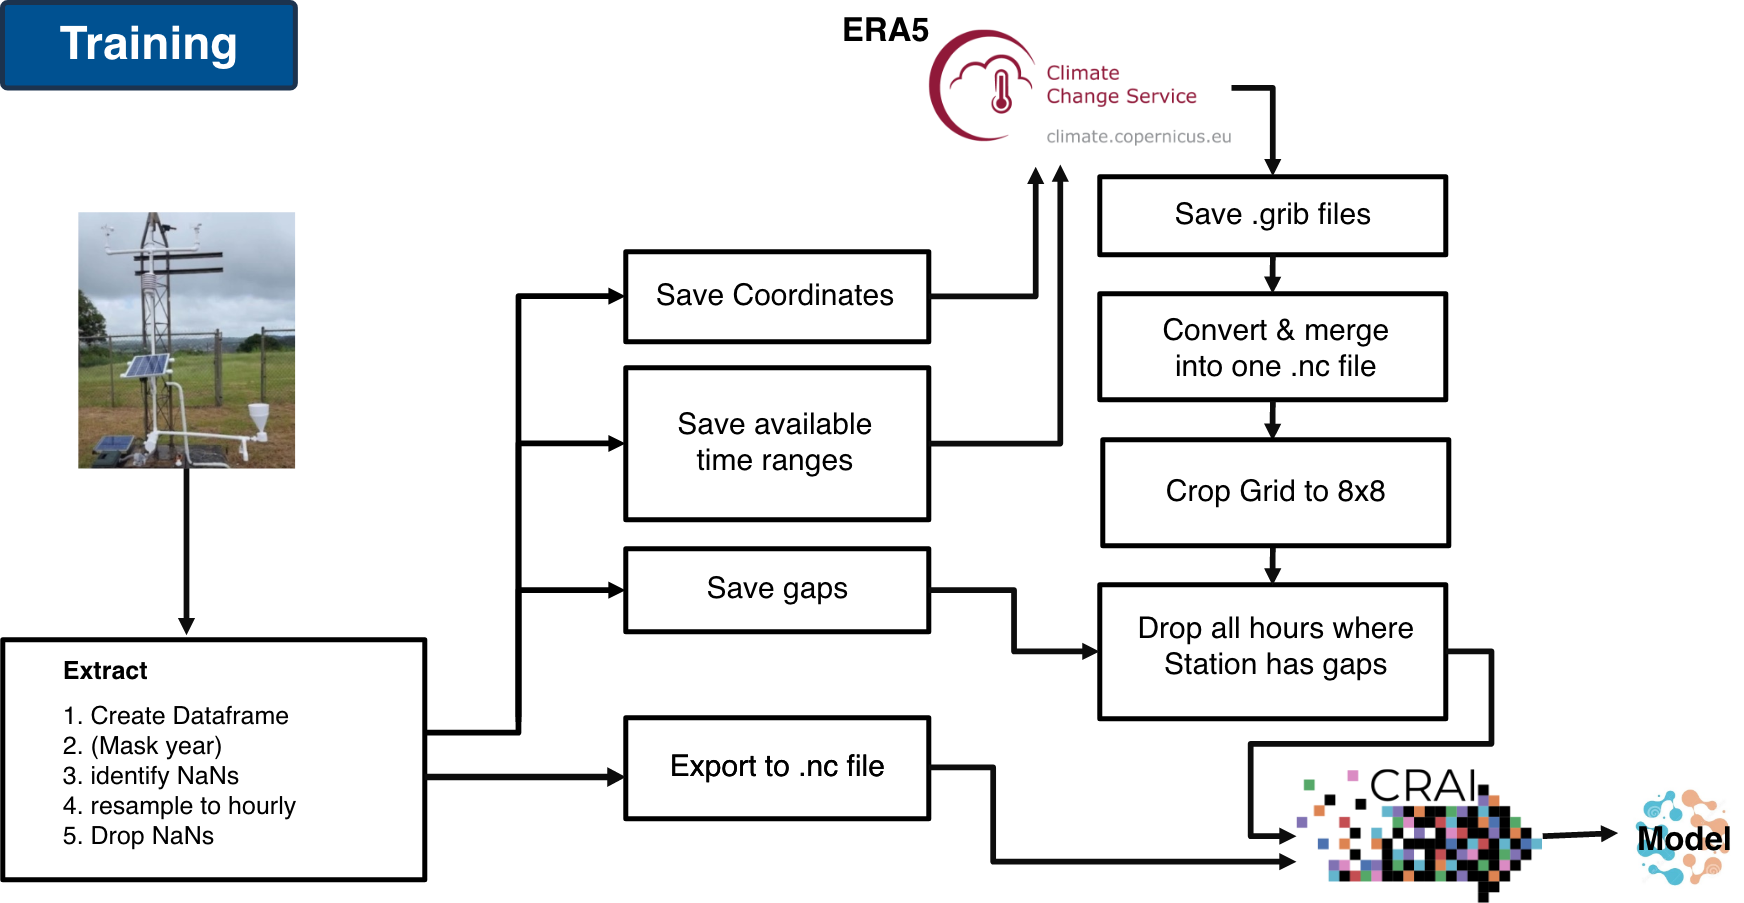
\includegraphics[width=450pt]{resources/images/training_pipeline.png}
    \caption{Pipeline to train a model}
    \label{fig:training_pipeline}
\end{figure}

\begin{figure}
    \centering
    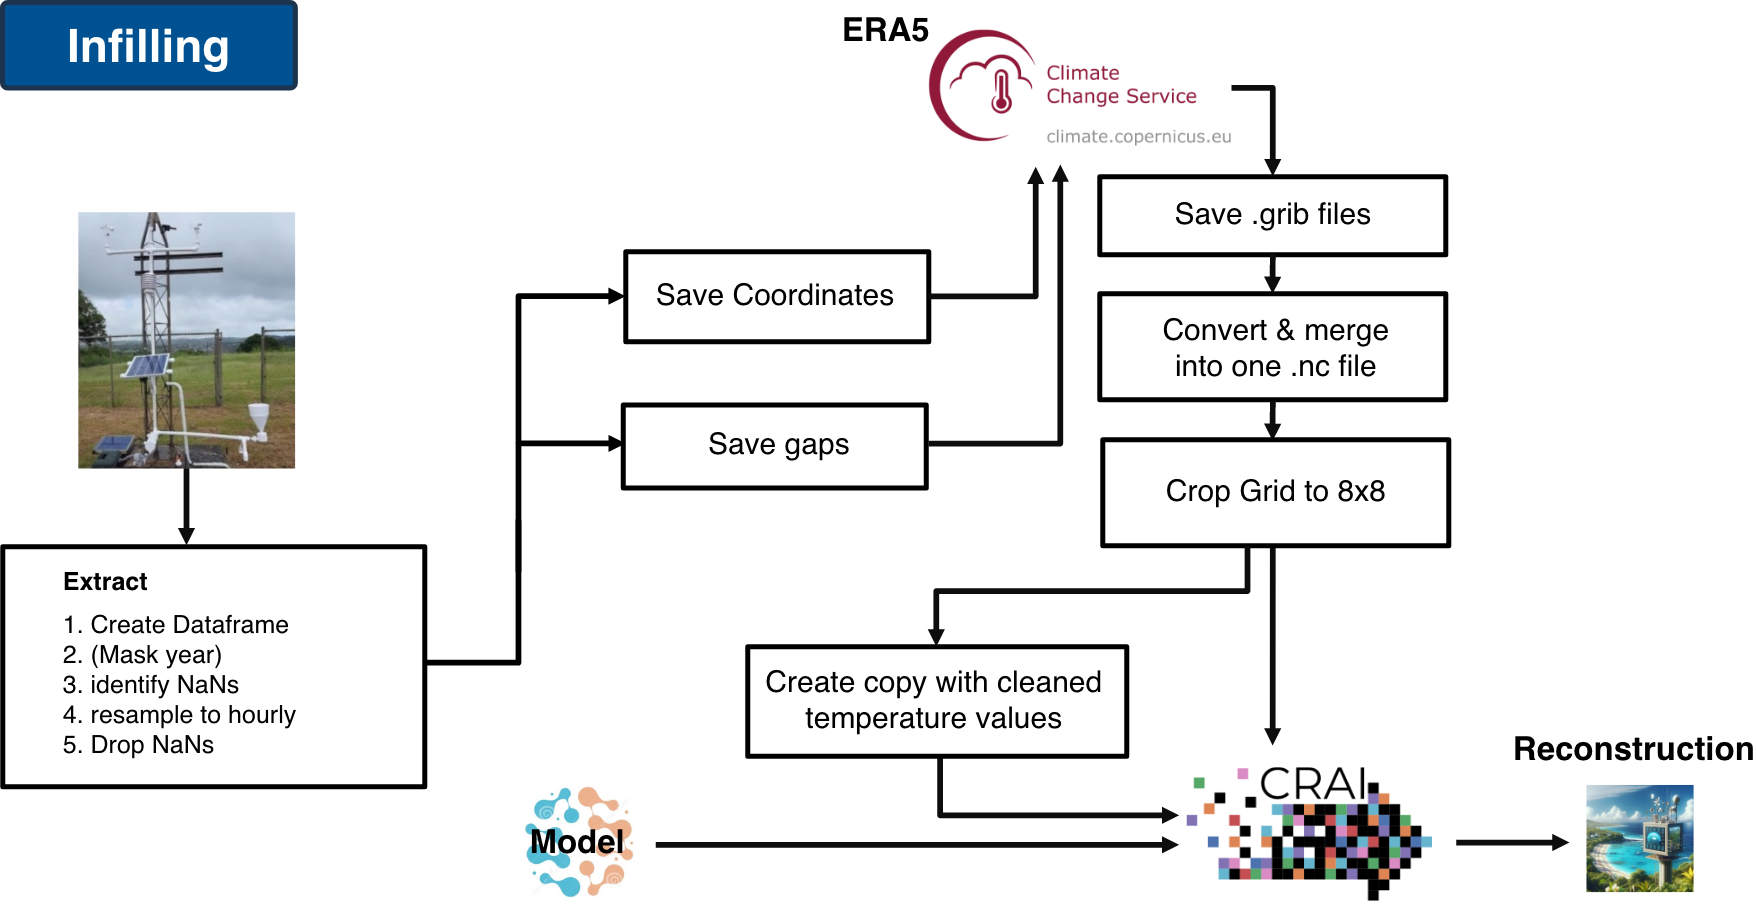
\includegraphics[width=450pt]{resources/images/infilling_pipeline.png}
    \caption{Pipeline to reconstruct weather data using a model}
    \label{fig:training_pipeline}
\end{figure}

\subsection{Stationdata Submission \& Conversion}

The station data for the 3D printed weather stations provided by NCAR comes in delimited text files, with one file per day and a text based metadata file holding information like the station name, the latitude and longitude and the elevation.
The data files (.dat files) hold per sensor one column and per minute one row.

A class "DatToNcConverter" is implemented with the following main use cases:
First to take in a directory with the .dat files and the metadata file and parse it. Second to process the data which is easiest in a pandas dataframe, dropping missing values and resampling to an hourly frequency, and converting from Celcius to Kelvin to match ERA5. Third to convert the data to a NetCDF file, which is the format that is used by the ERA5 data and the CRAI module. The NetCDF file is structured in a way that the data is stored in a 3D array with the dimensions time, latitude and longitude. The metadata is stored as global attributes in the NetCDF file. Fourth to convert some dataframe back to a .dat file after the reconstruction of measurements to match the original format when infilling. Of these use cases the one resampling to hourly frequency is the most complex, or at least could include many design decisions. Missing values are marked with "-999.99", so in the first step, these values can be marked as NaN. However, the data quality is by default not controlled and there could be values that should be marked as missing but are not. Thus the NCAR consulted to mark "0.00" °C as NaN. For stations like Barbados this wouldn't be a realistic value anyway, but even for regions where 0°C degrees are reached often, it's unlikely to measure exactly "0.00", meaning the amount of correct data lost through marking "0.00" as NaN is still limited. Also by agreement with the NCAR everything above or under +/- 45°C is marked as NaN. Additionally to compensate for peaks in the data aggregating the minutes using a median instead of a mean can be a good idea, numpy.median() would return NaN if any value is NaN and numpy.nanmedian() would ignore NaNs. It would be best to have a custom aggregate function using numpy.nanmedian() but assuring prior to that that there are sufficient non-NaN values.

For the usecase of converting the data back to a .dat file, the dataframe is stored directly in the converter object as original dataframe after detecting NaNs and resampling to hourly values, before any transformation of units (Celcius to Kelvin) or renaming of columns takes place and before NaNs are dropped. Fundamentally inbetween the first and last measurements rows for all minutes exist, even if measurements are missing. However if the station had severe issues it's possible that between first and last record there are even rows or files missing. To assure that the original dataframe will have rows for all hours, a handy method provided by the python pandas module is used:

\begin{lstlisting}
    self.original_df = self.original_df.reindex(
        pd.date_range(start = self.dataframe.index.min(), end = self.dataframe.index.max(), freq = "h"))
\end{lstlisting}

A class "Station" is implemented to hold the metadata and the pandas dataframe of the station data. It holds the converter itself, to minimize lines of code in the main script. The class is mainly used to manage the access to the different files and data, before and after the conversion. And secondly to detect the gaps in the data, for infilling simply in the form of listing the hours where data is missing. And for training use cases additionally in form of listing the months where at least some data is available which is most convenient for the API applicance to get ERA5 data for the station.


\begin{lstlisting}[caption=Gap Detection in Station Class, label=lst:find_gaps]
def find_gaps(self) -> None:
available_hour_steps = self.df.index
all_hour_steps = self.converter.original_df.index
# find all hours between the first and last hour that are missing
missing_hours = all_hour_steps.difference(available_hour_steps)
return missing_hours.tolist()
\end{lstlisting}

\begin{lstlisting}[caption=Detection of available ranges in Station Class, label=lst:available_ranges]
def get_all_months_in_df(self) -> None:
# return all (year, month) tuples in the dataframe
periods = self.df.index.to_period('M').unique().tolist()
month_dict = {}
for period in periods:
    if period.year not in month_dict:
        month_dict[period.year] = []
    month_dict[period.year].append(period.month)
return month_dict
\end{lstlisting}

\subsection{Copernicus Climate Data Store - CDS API}
\label{sec:cds_api}

The Copernicus Climate Data Store (CDS) is a service by the European Centre for Medium-Range Weather Forecasts (ECMWF). The CDS API provides opensource access to the ERA5 data, allowing users to download the data for a specific location and time period. After creating an account online an API Key can be obtained for free and with the python module 'cdsapi' data can be downloaded then easily in .grib format. 

\begin{lstlisting}[caption=Download Hook for ERA5 Data, label=lst:download_hook]
import cdsapi

class Era5DownloadHook:
    
    def __init__(self, lat, lon):
        self.cds = cdsapi.Client(
            url="https://cds.climate.copernicus.eu/api/v2",
            key=f"{os.getenv('UID')}:{os.getenv('API_KEY')}"
        )
        self.lon, self.lat = lon, lat

    def _download(cds, date_info, save_to_file_path):
        cds.retrieve(
        'reanalysis-era5-single-levels',
        {
            "product_type": "reanalysis",
            "format": "grib",
            "variable": "2m_temperature",
            "area": [
                self.lat + 1, # limit north
                self.lon - 1 % 360, # limit west
                self.lat - 1, # limit south
                self.lon + 1 % 360, # limit east
            ],
            "year": date_info.get("years"),
            "month": [f"{month:02d}" for month in date_info.get("months")],
            "day": [f"{day:02d}" for day in date_info.get("days")],
            "time": [f"{hour:02d}:00" for hour in date_info.get("hours")]

        }, save_to_file_path)



\end{lstlisting}

As seen in the code snippet, the request needs to include besides basic informations such as variable / format / model, the regional selection and the selection in the time dimension.
to download a few hours in a day the following can be used. When building requests that download a month or a full year, it becomes obvious why the \autoref{lst:available_ranges} is so useful.

\begin{lstlisting}[caption=Download Hours in Same Day in Download Hook Class, label=lst:download_hours_in_same_day]
    def download_hours_in_same_day(self, year, month, day, hours, target_folder):
        self.download({
            "years": [year],
            "months": [month],
            "days": [day],
            "hours": hours
        }, f"{year}_{month}_{day}.grib")
\end{lstlisting}

In the \autoref{lst:download_hook} it can be seen that the regional selection is always +/- 1 degree around the Station location. This ensures because of the grid interval of 0.25° that the downloaded area always includes at least 9x9 grid points, such that when cropping to an 8x8 selection the station can always be centered, even without exact knowledge of the coordinates of the desired grid points prior requesting. 


\subsection{Data Preprocessing}

As pointed out in \autoref{sec:cds_api} the data is downloaded in .grib format. Using the program 'cdo' the data can be quickly converted to .nc format. With the following simple command

\begin{lstlisting}
cdo -f nc copy {source_path} {nc_path}
\end{lstlisting}

However to have the temperature at surface variable name unified as "tas" in the NetCDF file, the following command can be used:

\begin{lstlisting}[caption=Renaming Variable in NetCDF File, label=lst:rename_variable]
    import xarray as xr
    import subprocess

    def _rename_variable(self, var_name, tas_name, input, output):
        rename_variable_command = \
            f"cdo chname,{var_name},{tas_name} {input_path} {output_path}"
        subprocess.run(rename_variable_command, shell=True)
        
    ds = xr.open_dataset(input_path)
    if 'var167' in ds.variables:
        _rename_variable('var167', 'tas', input_path, output_path)
    elif '2t' in ds.variables:
        _rename_variable('2t', 'tas', input_path, output_path)

\end{lstlisting}

Then the files are merged using 

\begin{lstlisting}
    cdo cat {temp_dir_path}/*.nc {era5_target_file_path}
\end{lstlisting}

before the data is cropped to the 8x8 grid around the station location, as described in \Ref{subsec:data_preprocessing}.

For training the data it needs to be assured that the ERA5 data does not include timesteps that the nc file of the station data does not include so that the time dimensions are identical. This is done in two steps, first the ERA5 data is cropped using a start / end date approach using the first and last date of the station data. Then all hours that were missing in the station dataset, identified by the find gaps method in \autoref{lst:find_gaps}, are removed from the ERA5 data. This is done usinfg the python module xarray and deleting the timesteps in batches of up to 1000 timesteps, as deleting all at once could cause issues.

The station data should have the same dimensions as the ERA5 data, so a method is applied that coppies the ERA5 dataset and replaces all the temperature values with the measured value from the corresponding hour in the station data.

For evaluating the model, in a validation procedure the same preparation of ERA5 data is done, however instead of passing the station data as expected output to the model, the file will not be filled with the measured values but with NaNs.

When evaluating the model not for validation but to infill missing values, the ERA5 data needs to be prepared differently of course. Instead of requesting monthly data from the cdsapi, it is requesing only the missing hours day by day, such that the timedimesion is directly as desired, and preprocessing only needs to handle conversion and geographical cropping.

\subsection{CRAI - Climate Reconstruction AI}

Because CRAI is using the encode, decode architecture with connected layers as described in \autoref{subsec:cnn}, the output file in NetCDF format that the model produces includes not only one temperature value per timestep but has the same dimensions as the input ERA5 file meaning it uses the same 8x8 grid with 64 temperature values. However since it has been trained on input files where the groudtruth was also laid on the 8x8 grid, the 64 temperature values in the output data of the model tend to be extremely similar. They need to be reshaped however to the original dimensions of the station data, which is a 1D array with 1 temperature value per timestep. This is done by taking the mean of the 64 values. 

\section{Process Orchestration + API \& Webinterface}

\subsection{Executer Classes, (Training, Infilling, Validation)}

\subsection{API Endpoints}

\subsection{Webinterface}

